% GUIDA VELOCE:
% --------------------------------------------------------------------
% X INIZIA UN UNOVO CAPITOLO:
% \chapter{??? NOME CAPITOLO}}
% \section{ ?? }
% \subsection{ ?? }
%
% --------------------------------------------------------------------
% PAROLA CONTENUTA NEL GLOSSARIO:
% scrivere la parola seguita da $^g$
% esempio: User$^g$
%
% --------------------------------------------------------------------
% PER ANDARE A CAPO SENZA RIENTRO INSERIRE:
% \\
%
% --------------------------------------------------------------------
% GRASSETO:
% \textbf{parola}
%
% --------------------------------------------------------------------
% CORSIVO:
% \emph{parola}
% --------------------------------------------------------------------
% PER SCRIVERE IN ROSSO:
% \red{parola}
%
% --------------------------------------------------------------------
% PER SCRIVERE TRA VIRGOLETTE
% ''parola''
%
% --------------------------------------------------------------------
% PER EVITARE IL RIENTRO AUTOMATICO DI UN CAPOVERSO:
% \noindent testo....
%
% --------------------------------------------------------------------

% PER SCRIVERE CARATTERI PARTICOLARI COME: { } _ ecc.. SCRIVERLI PRECEDUTI DA \
% ES: \{ \_
%
% --------------------------------------------------------------------
% X INSERIRE UN LINK:
% \url{http://www.math.unipd.it/~tullio/IS-1/2011/Progetto/C3.pdf}
%
% --------------------------------------------------------------------
% PER COMMENTARE INTERE PARTI:
% \comment{ comment }
%
% --------------------------------------------------------------------
% PER SCRIVERE NOTE DURANTE IL TESTO:
% parola \footnote{ note riguardanti la parola }
%
% --------------------------------------------------------------------
% PER SCRIVERE CODICE SORGENTE:
%
% \lstset{language=c++,
% stringstyle=\color{blue}\textrm,
% commentstyle=\rmfamily, numbers= none}

% \begin{lstlisting}
% CODICE
% \end{lstlisting}
%
% --------------------------------------------------------------------
% !!!!!!!! PER COSE + COMPLESSE VEDI: !!!!!!!!!!!!!!!!!!!!!!!
% !!!!!!!! PMAC/latex/GUIDA LATEX!!!.tex !!!!!!!!!!!!!!!!!!!!!!!

% per tutto il resto chiedi a lory prima di fare/scrivere cazzate !!!!!!!!!!



\documentclass[10pt,a4paper]{book}

\usepackage[italian]{babel}
\usepackage[T1]{fontenc}
\usepackage[utf8x]{inputenc} % uso utf8x xk x linux, mentre latin1 è per windows
\usepackage{lmodern} %insieme di font molto completo consigliato da LatexFacile pg13 in basso
\usepackage{microtype} %migliora riempimento delle righe. vedi LatexImpaziente pg41
%attiva il rientro di ogni prima riga di ogni sezione: capitolo,paragrafo ecc. vd LatexImpaziente pg41
\usepackage{indentfirst}
\usepackage{graphicx} % per inseire immagini
\usepackage[usenames,dvipsnames]{color}
\usepackage{lastpage} %serve per poter scrivere page 1 of N
% setta i bordi della pagina: dx e sx 3.2cm di rientro + nel lato di rilagatura rientra di altri 0mm
\usepackage[a4paper,top=3cm,bottom=3cm,left=3.2cm,right=3.2cm, bindingoffset=0mm]{geometry}
\usepackage{listings} % per inserire codice sorgente
\usepackage{float} % per gestire oggetti flottanti ( es immagini tabelle posizionebili con "H" che forza il posizionamento nel punto specifico )

% serve per creare tabelle lunghe + di una pagina con \begin{longtable} (vd Tabelle.pdf pg11-12)
\usepackage{longtable}
\usepackage{marvosym} % per l' \EUR

\usepackage{fancyhdr} % per impostare lo stile della pagina più personalizzato, + fancyhdr ( per regolare testatina e piè di pagina ) vedi itfancyhrd



\pagestyle{fancy}
% settaggi di pagestyle(fancy)
\lhead{
\includegraphics[scale=0.20]{images/SevenFold_small}}
%\chead{}
\rhead{\textbf{{%
\NomeDocumento - \VersioneAttuale \\ Data versione attuale: \DataRilascio \\ e-mail: \mail{sevenfold@palomino.it}}}}
\lfoot{\NomeDocumento}
\cfoot{}
\rfoot{ \textbf \thepage\ di \pageref{LastPage}}
\renewcommand{\footrulewidth}{0.4pt}

%ridefinisco il plain per cosare l'indice (a questo punto si potrebbe lasciare tutto il documento in plain
\fancypagestyle{plain}{
\lhead{
\includegraphics[scale=0.20]{images/SevenFold_small}}
%\chead{}
\rhead{\textbf{{%
\NomeDocumento - \VersioneAttuale \\ Data versione attuale: \DataRilascio \\ e-mail: \mail{sevenfold@palomino.it}}}}
\lfoot{\NomeDocumento}
\cfoot{}
\rfoot{ \textbf \thepage\ di \pageref{LastPage}}
\renewcommand{\footrulewidth}{0.4pt}
}

% da ultimo:
\usepackage{hyperref} %x l'interpretazione di indirizzi o link ipertestuali (vd LatexImpaziente pg47 )
\hypersetup{backref, colorlinks=true, linkcolor=black, urlcolor=black}

\usepackage{url} % x l'interpretazioni di internet o link ipertestuali (vd LatexImpaziente pg47 )
%\UrlFont{color =blue}
%\urlstyle{helvetic}

% Define a new 'leo' style for the package that will use a smaller font.
\makeatletter
\def\url@leostyle{%
  \@ifundefined{selectfont}{\def\UrlFont{\sf}}{\def\UrlFont{\small\ttfamily}}}
\makeatother
%% Now actually use the newly defined style.
\urlstyle{leo}


\newcommand{\mail}[1]{\textcolor{Black}{ \texttt{#1}}} %per interpretare mail (vd LatexImpaziente pg47 )
\newcommand{\cambiaFont}[2]{{\fontencoding{T1}\fontfamily{#1}\selectfont#2}}
\newcommand{\red}[1]{ \textcolor{red}{#1} } % per scrivere testo in rosso
\newcommand{\comment}[1]{} % per inserire commenti

\newcommand{\attribute}[2]{ \item[\textcolor{PineGreen}{ \texttt{#1}}] \textcolor{PineGreen}{\texttt{#2\\}}\ \ \ }
\newcommand{\method}[2]{ \item[\textcolor{MidnightBlue}{ \texttt{#1}}] \textcolor{MidnightBlue}{ \texttt{#2\\}}\ \ \ }

\newcommand{ \class}[1]{ \item[-] \texttt{#1} }
\newcommand{\virgolette}[1]{``{#1}''}



% INSERIRE QUI IL NOME DEL DOCUMENTO SEGUITO DA UNO SPAZIO
% ( così il nome si imposta in automatico nelle varie ricorrenze standard)
\newcommand{\NomeDocumento}{Scrivi in questo documento k poi uniamo tutto }

% INSERIRE QUI LA DATA DEL RILASCIO DELLA VERSIONE ATTUALE
\newcommand{\DataRilascio}{2012/04/02}

% INSERIRE LA VERSIONE ATTUALE
\newcommand{\VersioneAttuale}{v2.0.0}

% INSERIRE QUI L'ACRONIMO DEL DOCUMENTO. ESEMPIO: Analisi Dei Requisiti = AR
% Quando inserite l'acronimo qui, dovete rinominare i file presenti nella cartella
% del tipo '??-cap1-NomeCapitolo.tex' sostituendo i '??' con l'acronimo scelto!!
\newcommand{\AcronimoDocumento}{DP}

\begin{document}


% --------------------------------------------------------------------

% TITOLO ( 1° pagina)

\vspace*{2.5cm}
\begin{center}

%\cambiaFont{Cyklop}{Sevenfold}
%\cambiaFont{fve}{\Huge{Sevenfold}}

\includegraphics[scale=0.35]{images/SevenFold_big}

\vspace{2cm}

\cambiaFont{fve}{\Huge{\NomeDocumento}}\\
\vspace*{1cm}

è richiesto: circa 15 pagine a testa..

\end{center}


% --------------------------------------------------------------------

% INFORMAZIONI DEL DOCUMENTO ( 1° pagina)

\vspace*{2cm}




% --------------------------------------------------------------------

% SOMMARIO ( 2° pagina)

\newpage

\vspace*{0.5cm} % il vertical space va preceduto da una riga vuota!!!
\begin{center}

\textbf{{\huge{Sommario}}}

Questo documento contiene la struttura del sistema Woty, analizzando nel dettaglio i suoi componenti.

\vspace*{0.2cm} % il vertical space va preceduto da una riga vuota!!!

\end{center}


% --------------------------------------------------------------------



% --------------------------------------------------------------------
% INDICI:

\newpage

% INDICE CAPITOLI
\tableofcontents % genera l'indice di tutto il documento

\let\cleardoublepage\clearpage % toglie la pagina bianca dopo l'indice

% INDICE TABELLE
\listoftables

% INDICE FIGURE
\listoffigures


% --------------------------------------------------------------------

% INTRODUZIONE ( 1° CAPITOLO ) QUESTO CAPITOLO VA MESSO IN OGNI DOCUMENTO!!!!!!!!

\newpage
\chapter{Analisi di mercato}

\section{Introduzione}

L'analisi sugli infortuni che segue si riferisce a dati relativi solo all'ambito italiano in quanto prevediamo una diffusione iniziale del software solo a livello nazionale.\\
Per un possibile ampliamento di mercato fare riferimento al capitolo Business Model.



%\subsection{Infortuni sul lavoro: statistiche}

\section{Bilanci infortunistici 2011}
Di seguito verranno riportati alcuni valori sugli infortuni sul lavoro registrati nell'ultimo decennio e in particolare verranno analizzati più dettagliatamente i valori registrati nel 2011.

\subsection{Visione genarale}


Ammontano a circa 920 i morti sul lavoro registrati nel 2011, pari a più di due persone ogni giorno.\\
Questo dato è in lieve calo rispetto ai 973 morti registrati nel 2010, ma nonostante ciò la cifra rimane ancora poco rassicurante.\\
Secondo il rapporto annuale dell'Inail anche gli infortuni sul lavoro registrati hanno visto un lieve calo, passando dai 776mila del 2010 agli 725mila del 2011, registrando una flessione del 6,6\%, pari a 51mila casi in meno.\\

\begin{figure}[H]
\centering
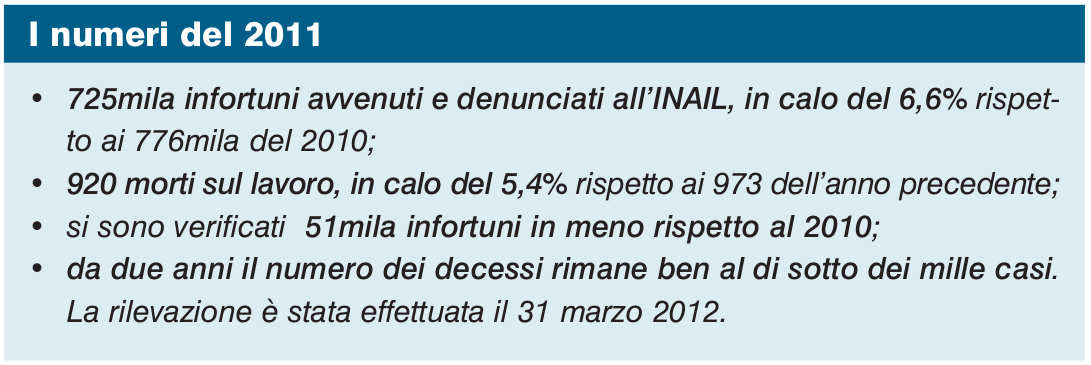
\includegraphics[scale=0.3]{images/analisiDiMercato/infortuniGenerale}
\caption{I numeri del 2011, fonti INAIL}
\end{figure}


In queste cifre non rientrano però gli infortuni relativi ai quasi 3 milioni (secondo i dati Istat) di lavoratori in nero presenti nel notro paese, tra i quali l’Istituto stima che nel 2010 (ultima proiezione disponibile) siano accaduti circa 164mila casi di infortunio.\\

\begin{figure}[H]
\centering
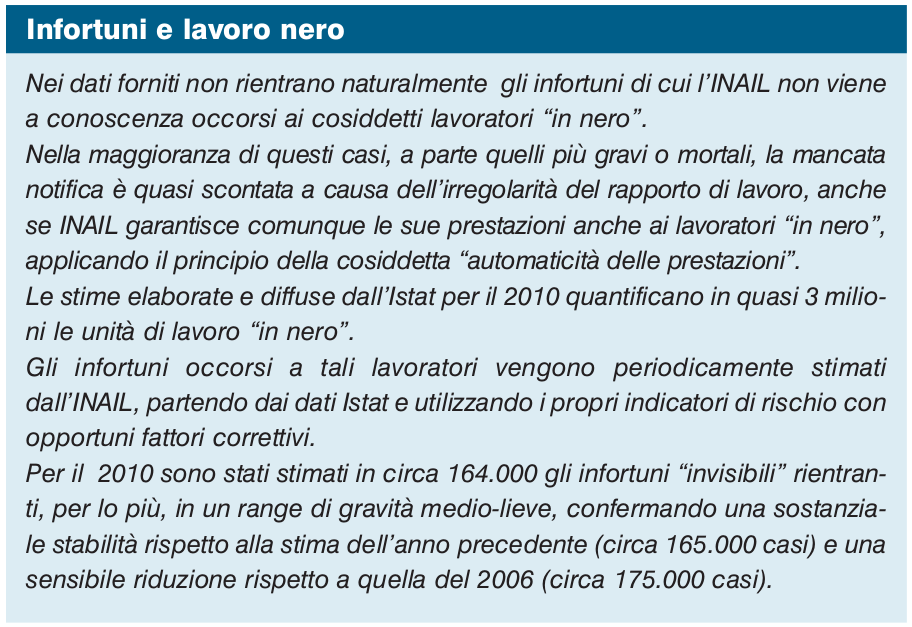
\includegraphics[scale=0.4]{images/analisiDiMercato/infortuniLavoroNero}
\caption{Infortuni e lavoro nero, fonti INAIL}
\end{figure}

Tra le 21.201 aziende controllate dall'Inail nel 2011, ben l’85,59\% è risultato ''irregolare'' per l’efficienza dei sistemi di scelta, della procedura cosiddetta di business intelligence che individua gli insiemi da controllare. Sono stati inoltre regolarizzati 48.716 lavoratori (nel 2010 erano stati 56.751), di cui 41.207 irregolari e 7.509 in nero (4.426 nel terziario, 2.675 nell’industria).\\\\



\
\
\
**business intelligence: un insieme di processi aziendali per raccogliere ed analizzare informazioni strategiche.\\\\

\ \
\subsection{Statistiche nel dettaglio}

\textbf{Infortuni per modalità di evento}\\
Per procedere in un’analisi dettagliata dei valori sugli infortuni sul lavoro, vanno prima di tutto distinte le modalità in cui avviene l’infortunio:

\begin{itemize}
\item \textbf{in occasione di lavoro} sono i casi che avvengono nell’esercizio effettivo dell’attività;
\item \textbf{in itinere} sono invece quelli che accadono al di fuori del luogo di lavoro, durante il per-
corso casa-lavoro-casa.
\end{itemize}


E' possibile notare una diminuzione tra il 2010 e il 2011 su entrambe le tipologie di infortuni:\\
negli infortuni in itinere si è registrata una flessione del 7,1\%, passando da 88.129 casi del 2010 a 81.861 nel 2011;\\
mentre negli infortuni avvenuti in occasione di lavoro, che rappresentano circa il 90\% del com-
plesso delle denunce, la flessione è stata invece pari a 6,5\%.\\
Da notare come ben il 90\% degli infotuni si concentri unicamente nei settori lavorativi riguardanti \textit{l'industria e i servizi}: questo dato può far riflettere molto sull'utilità di sviluppare una buona prevenzione sugli infortuni sul lavoro mirata soprattutto a quensti settori fortemente a rischio.\\
Il restante 10\% degli incidenti invece è ripartito per il 6\% nel settore \textit{agricolo} e per il 4\% tra i \textit{dipendenti del conto Stato}.


\begin{figure}[H]
\centering
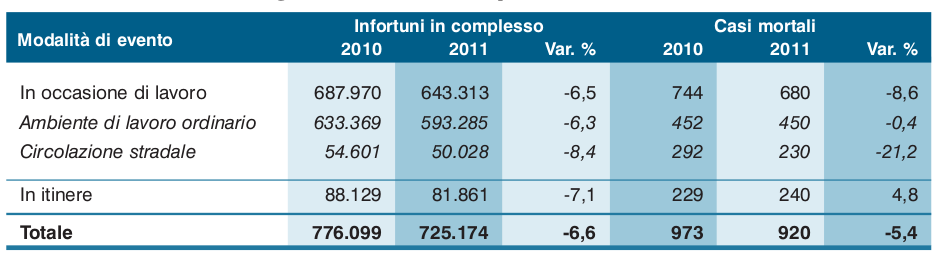
\includegraphics[scale=0.5]{images/analisiDiMercato/infortuniPerModalita}
\caption{Infortuni denunciati 2010-2011, per modalità di evento}
\end{figure}


\textbf{Infortuni per attività}\\
Dall’analisi settoriale si può notare come nel 2011 la diminuzione degli infortuni sul lavoro, rispet-
to all’anno precedente, abbia interessato in primo luogo il settore dell’Industria (-8,2\%), dell’Agricoltura (-6,5\%) e le attività dei Servizi (-5,5\%), che sono i tre settori con il maggior numero di infortuni.
Durante lo stesso periodo va segnalata però, secondo i dati Istat, una diminuzione degli occupati nell’Industria dello 0,6\% e nell’Agricoltura dell’1,9\% e, viceversa, una leggera ripresa nei Servizi (+1\%).
Tra le attività nel dettaglio, si distinguono per una elevata riduzione degli infortuni le
Costruzioni (-14,7\%) a fronte di un calo occupazionale del 5,3\%, seguite con un più con-
tenuto ma significativo calo da importanti settori quali la Meccanica (-6,7\%) e la
Metallurgia (-6,6\%).
Nei Servizi la diminuzione degli infortuni è ha riguardato in maggior modo i settori
più rilevanti dal punto di vista dimensionale: Trasporti (-11,3\%), Servizi alle imprese e atti-
vità immobiliari (-9,7\%), Commercio (-9,6\%). Anche per il settore del personale addetto
ai servizi domestici si segnala un calo contenuto del 3,4\%.
Per quanto riguarda i casi mortali, analizzando le attività nel dettaglio, si è registrato nel
2011 una diminuzione sensibile dei Servizi (-9,4\%) e dell’Industria (-3,7\%), mentre per
l’Agricoltura si segnala un +2,7\%. Tra i settori più rilevanti, una riduzione molto elevata
si è verificata nei Trasporti (-30,7\%), nei Servizi alle imprese e attività immobiliari (-26,2\%)
e le Costruzioni (-10,6\%). Viceversa, sono aumentate le vittime nell'ambito dell’ Industria pesante della Metalmeccanica.\\\\


\begin{figure}[H]
\centering
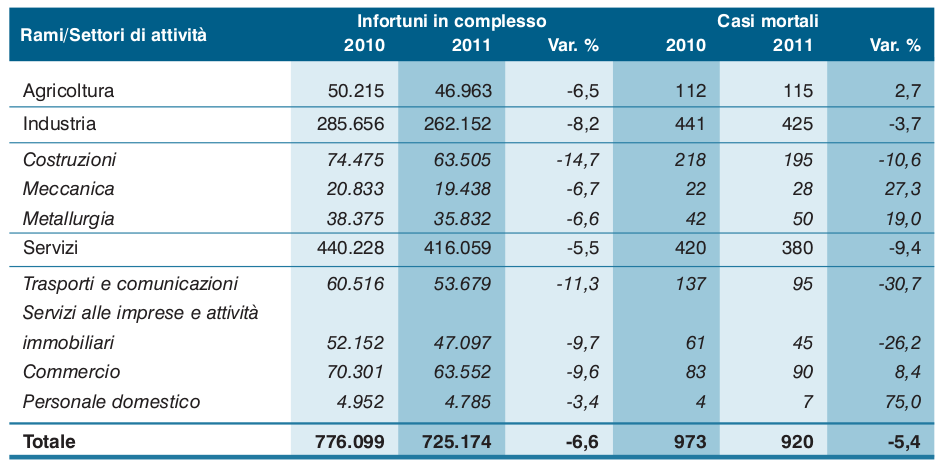
\includegraphics[scale=0.5]{images/analisiDiMercato/infortuniPerGestione2}
\caption{Infortuni denunciati 2010-2011, per settori e attività}
\end{figure}








\textbf{Infortuni per sesso}\\
Nel 2011 il calo infortunistico ha interessato sia i lavoratori (-7,0\%) che le
lavoratrici (-5,6\%).\\
Per quanto riguarda invece il calo complessivo degli infortuni mortali  (-5,4\%), questa flessione è influenzata esclusivamente dei lavoratori di sesso maschile, poichè al contrario, gli infortuni mortali sul lavoro del sesso femminile, hanno riscontrato un sensibile aumento dei decessi (+15,4\%, passando dai 78 casi del 2010 ai 90 del 2011). Tale aumento è dovuto prevalentemente ai casi in itinere che rappresentano più della metà dei decessi femminili.
Per questi valori, va considerato che, secondo i dati Istat, le donne rappresentano circa il 40\% degli
occupati, e che la quota di infortuni femminili rispetto al totale è del 32\% e quasi il 10\% per
i casi mortali. Da questo \textit{si deduce che il lavoro femminile è sicuramente meno rischioso}; le donne
sono, infatti, occupate prevalentemente nei servizi e in settori a bassa pericolosità e, se
impegnate in comparti più rischiosi come quello delle Costruzioni, dei Trasporti e
dell’Industria pesante, svolgono comunque mansioni di tipo impiegatizio o dirigenziale.


\begin{figure}[H]
\centering
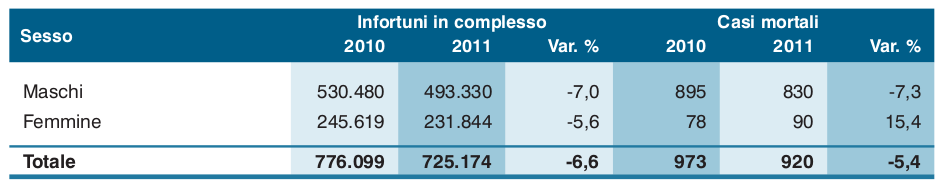
\includegraphics[scale=0.5]{images/analisiDiMercato/infortuniPerSesso1}
\caption{Infortuni denunciati 2010-2011, per sesso}
\end{figure}

\begin{figure}[H]
\centering
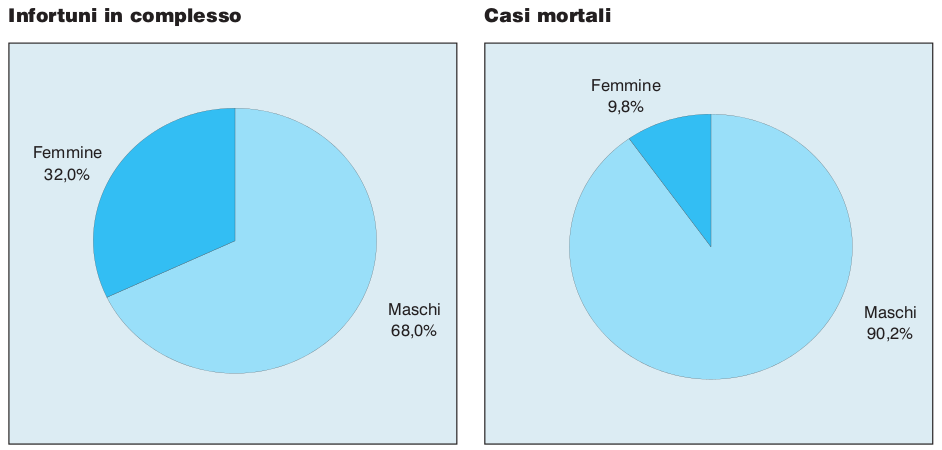
\includegraphics[scale=0.5]{images/analisiDiMercato/infortuniPerSesso2}
\caption{Infortuni per sesso, anno 2011}
\end{figure}

\textbf{Infortuni per età}\\
Analizzando i dati per fascia di età, è facile notare che la fascia tra i 35-49 risulta la più colpita con ben il 44\% di tutti gli infortuni, mentre la seconda fascia di età più colpita risulta essere quella fino ai 34 anni, con il 32\% degli infortuni complessivi.

\begin{figure}[H]
\centering
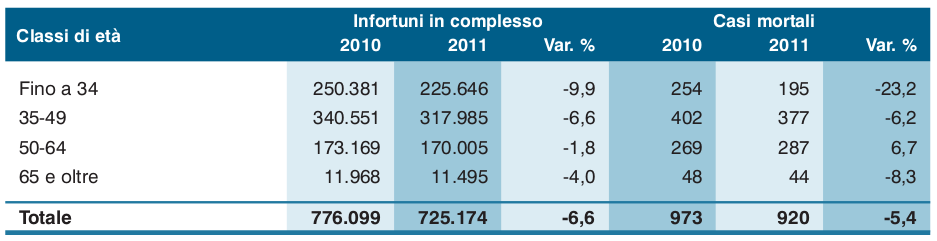
\includegraphics[scale=0.5]{images/analisiDiMercato/infortuniPerEta1}
\caption{Infortuni denunciati 2010-2011, per età}
\end{figure}

\begin{figure}[H]
\centering
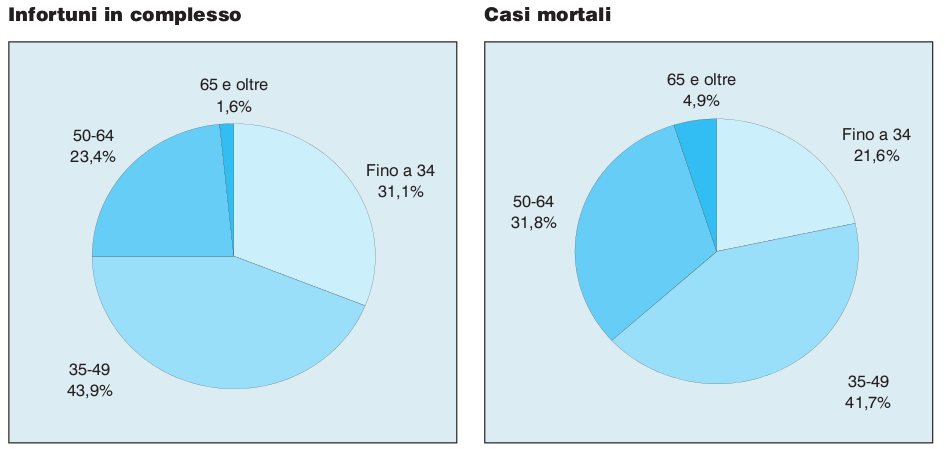
\includegraphics[scale=0.53]{images/analisiDiMercato/infortuniPerEta2}
\caption{Infortuni per età, anno 2011}
\end{figure}







\ \ \
\section{Bilanci infortunistici ultimo decennio 2002-2011}
\ \
\subsection{Visione genarale}

Ampliando l'osservazione dei dati sugli infortuni sul lavoro all'ultimo decennio, si può notare come il calo registrato nel 2011, rientri in un andamento decrescente delle denunce di infortunio:
\begin{itemize}
\item tra il 2002 e il 2011 le denunce sono scese da 992.665 a 725.174;
\item la contrazione complessiva è stata del 26,9\% (circa 268.000 infortuni in meno).
\end{itemize}



\ \
\subsection{Statistiche nel dettaglio}

\textbf{Infortuni per attività}\\
Scomponendo il fenomeno secondo i tre grandi rami di attività previsti dalla classifica-
zione Istat, si registra, dal 2002 al 2011, una diminuzione degli infortuni sul lavoro sensibile e costante in Agricoltura (pari a -36,1\%) e nell’Industria (-44,0\%). Anche nei
Servizi, dopo anni di sostanziale stabilità, la riduzione è divenuta apprezzabile (-7,8\%).



\begin{figure}[H]
\centering
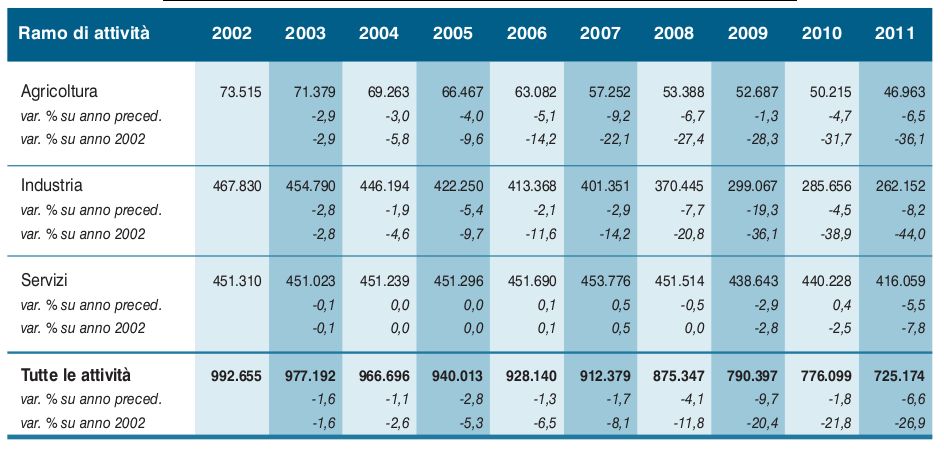
\includegraphics[scale=0.5]{images/analisiDiMercato/infortuniDecennioPerGestione1}
%\caption{Infortuni per attività, decennio 2002-2011}
\end{figure}

\begin{figure}[H]
\centering
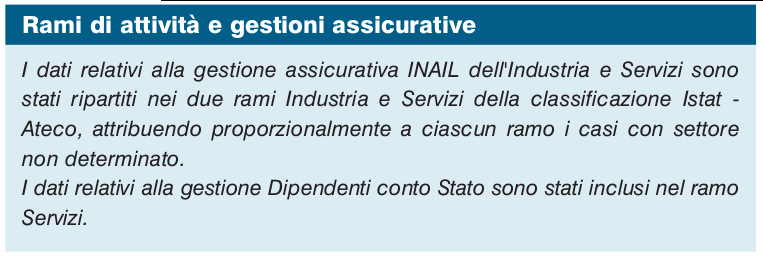
\includegraphics[scale=0.55]{images/analisiDiMercato/infortuniDecennioPerGestione2}
\caption{Infortuni per attività, decennio 2002-2011}
\end{figure}



\textbf{Infortuni per modalità}\\
La flessione ha riguardato esclusivamente gli infortuni in occasione di lavoro ( cioè durante il reale
ambito lavorativo):\\
tra il 2002 (920.299 denunce) e il 2011 (643.313 denunce) gli infortuni in occasione di
lavoro hanno fatto registrare un consistente calo di oltre il 30\%.\\

Nello stesso periodo, invece, gli infortuni in itinere sono passati dai 72.356 casi denunciati del 2002 agli 81.861 del 2011 con una crescita del 13,1\%, anche se già a partire dal
2009 (92.926 casi) si assiste ad un calo dei casi, dopo anni di costante aumento.
La quota di infortuni in itinere sul totale degli infortuni è aumentata nel decennio, dal
7,3\% del 2002 all’11,3\% del 2011.


\begin{figure}[H]
\centering
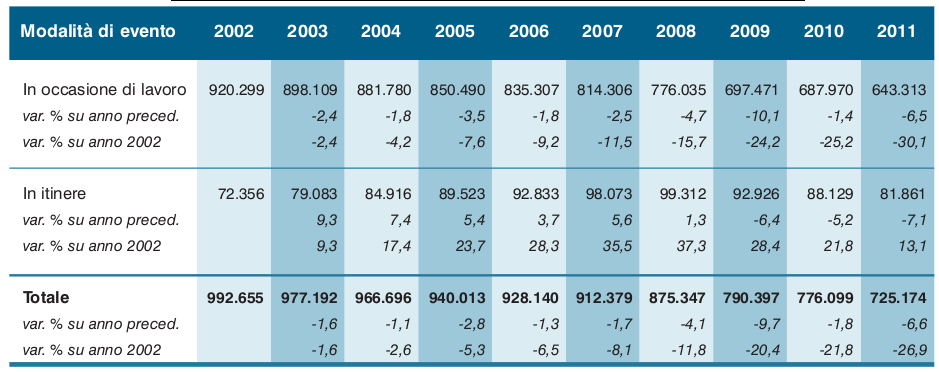
\includegraphics[scale=0.55]{images/analisiDiMercato/infortuniDecennioPerModalita}
\caption{Infortuni per modalità, decennio 2002-2011}
\end{figure}




Nel periodo 2002-2011, a livello di singolo ramo di attività è possibile notare le seguenti variazioni significative:
\begin{itemize}
\item l’Industria detiene ancora il risultato migliore, con una contrazione complessiva dell’indice di incidenza del 42,6\% (calo degli occupati registrato dall’Istat del 2,4\%);
\item l’Agricoltura segue con -25,6\% (calo degli occupati del 14,1\%);
\item inferiore il calo del ramo Servizi (-15,8\%), che è il solo comunque a beneficiare di
un positivo andamento nelle dinamiche occupazionali (crescita del 9,5\%).\\
\end{itemize}


\textbf{Infortuni mortali}\\
Anche per quanto riguarda gli infortuni mortali, nel periodo 2002-2011 si conferma una costante decrescita e le serie storiche rivelano gli enormi progressi compiuti dai primi anni sessanta, quando si toccò nel 1963, in pieno boom economico il tragico record storico di 4.664 morti in un solo anno.
Più in dettaglio, il calo dei morti sul lavoro, registrato nel decennio di interesse, risulta molto
sostenuto in tutti e tre i grandi rami di attività:
\begin{itemize}
\item Agricoltura -31,1\%,
\item Industria -41,3\%,
\item Servizi -35,3\%).\\
\end{itemize}

Le difformità tra i rami sono da attribuire, alla diversa dinamica occupazionale che ha registrato nel periodo osservato, un calo del 14,1\% in Agricoltura, un calo più modesto nell’Industria (-2,4\%) e una crescita del 9,5\% nei Servizi.



\begin{figure}[H]
\centering
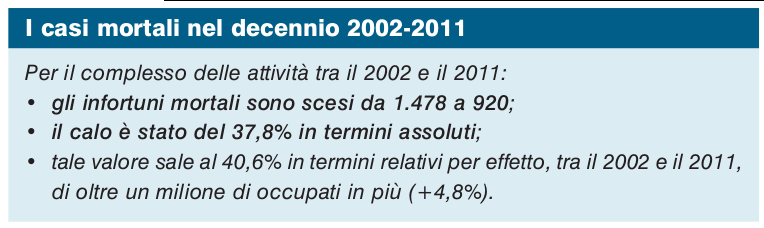
\includegraphics[scale=0.5]{images/analisiDiMercato/infortuniDecennioPerMortalita1}
\caption{Infortuni per mortalità, decennio 2002-2011}
\end{figure}

\begin{figure}[H]
\centering
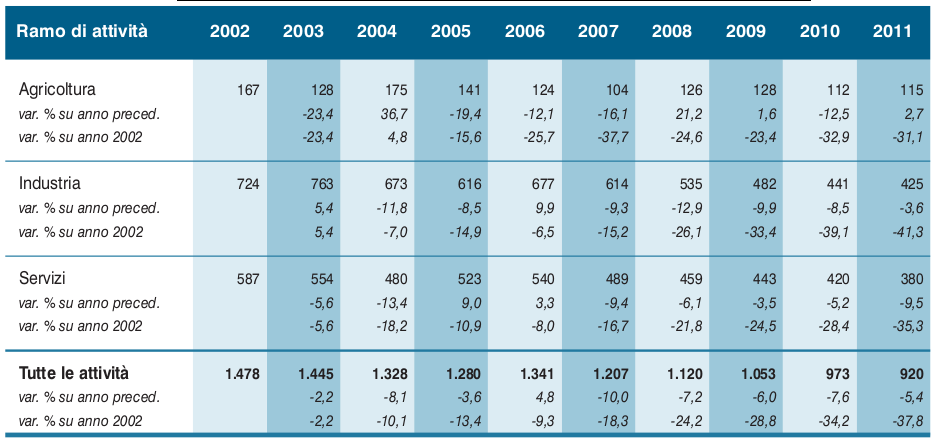
\includegraphics[scale=0.55]{images/analisiDiMercato/infortuniDecennioPerMortalita2}
\caption{Infortuni per mortalità riassunto, decennio 2002-2011}
\end{figure}





\textbf{Infortuni mortali per modalità}\\
Per gli eventi mortali è importante disinguere tra i decessi avvenuti nello
svolgimento della propria mansione lavorativa (in occasione di lavoro) e quelli in itinere
(gli infortuni avvenuti in genere nel percorso di spostamento casa-lavoro-casa).
La distinzione è importante poichè si può ragionevolmente ritenere che i decessi in
itinere non siano strettamente collegati alla specifica attività svolta dall’infortunato e quin-
di richiedano anche una diversa valutazione nella lettura del rischio che determina il
fenomeno infortunistico.



\begin{figure}[H]
\centering
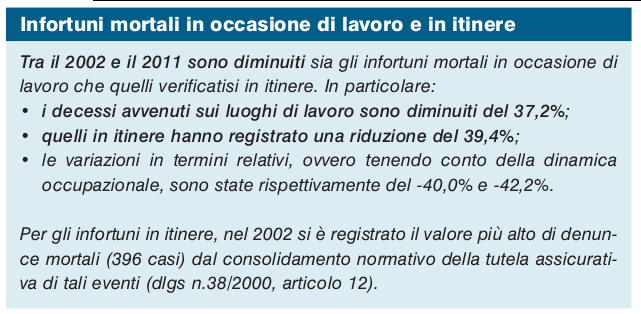
\includegraphics[scale=0.55]{images/analisiDiMercato/infortuniDecennioMortaliPerModalita1}
\caption{Infortuni mortali per modalità riassunto, decennio 2002-2011}
\end{figure}

\begin{figure}[H]
\centering
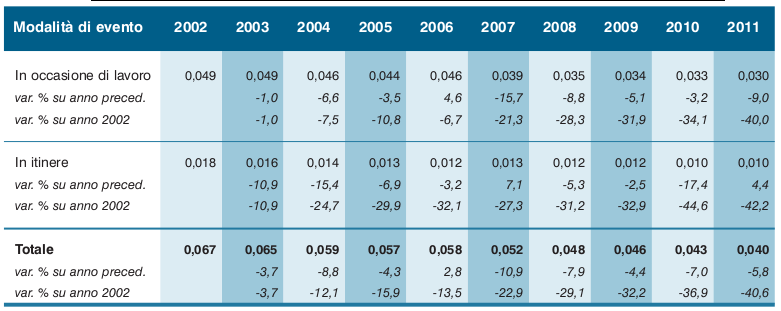
\includegraphics[scale=0.65]{images/analisiDiMercato/infortuniDecennioMortaliPerModalita2}
\caption{Infortuni mortali per modalità, decennio 2002-2011}
\end{figure}



\textbf{Infortuni per nazionalità}\\
Dagli ultimo dati Istat, è emerso che gli stranieri residenti in Italia al 1° gennaio 2011 sono
4.570.317, 335 mila in più rispetto all’anno precedente (+7,9\%).\\
Questi cittadini rappresentano un valore molto influente sui dati sugli infortuni sul lavoro, considerando che nel 2011 i lavoratori stranieri assicurati all’INAIL sono stati circa 3 milioni, valore che ha visto un incremento dell’1,3\% in più rispetto all'anno precedente e del 17,8\% in più del 2007.\\


\begin{figure}[H]
\centering
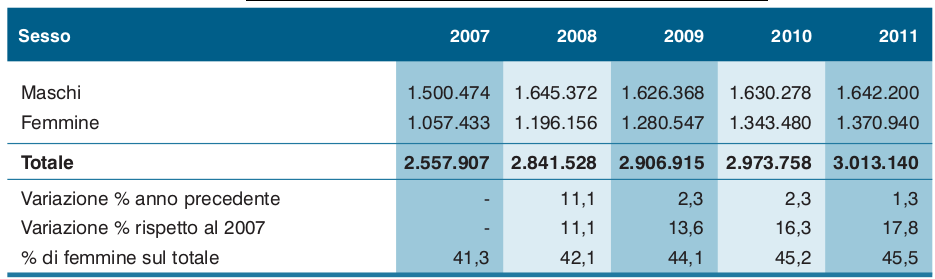
\includegraphics[scale=0.55]{images/analisiDiMercato/lavoratoriStranieri1}
\caption{Lavoratori stranieri assicurati all’INAIL per sesso}
\end{figure}

\begin{figure}[H]
\centering
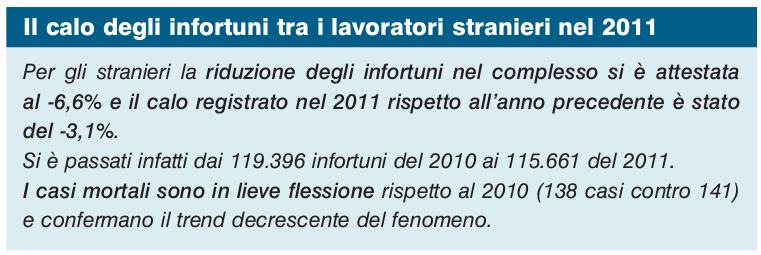
\includegraphics[scale=0.55]{images/analisiDiMercato/lavoratoriStranieri2}
\caption{Infortuni nei lavoratori stranieri}
\end{figure}



Gli infortuni degli stranieri rappresentano il 15,9\% degli infortuni complessivi, quelli dei
soli extracomunitari, invece, l’11,7\%; se si considerano i casi mortali le percentuali sono
rispettivamente del 15\% e dell’ 8,8\%.\\
In generale risulta che il 94,3\% degli infortuni degli stranieri si verifica nell’Industria e
servizi, il 5\% in Agricoltura e lo 0,7\% tra i Dipendenti conto Stato.\\
Da questi dati possiamo ricavare che non deve essere sottovalutata la fascia di lavoratori stranieri presente nel nostro paese in quanto rappresenta una percentuale non esigua e lo stesso va affermato per il numero di infortuni occorsi.\\



\textbf{Infortuni e indennizzi}\\
Gli infortuni indennizzati ogni anno dall'Inail sono circa 500.000 ogni anno, con una flessione che va da 650.000 nell'anno 2007, ai 478.000 nel 2011.\\
E' pertanto ipotizzabile che le somme di denaro spese dall'Inail per gli indennizzi sugli infortuni sul lavoro siano ingenti.\\
Di seguito viene riportato un rapporto sul numero degli infrotuni indennizzati nell'ultimo quinquennio:

\begin{figure}[H]
\centering
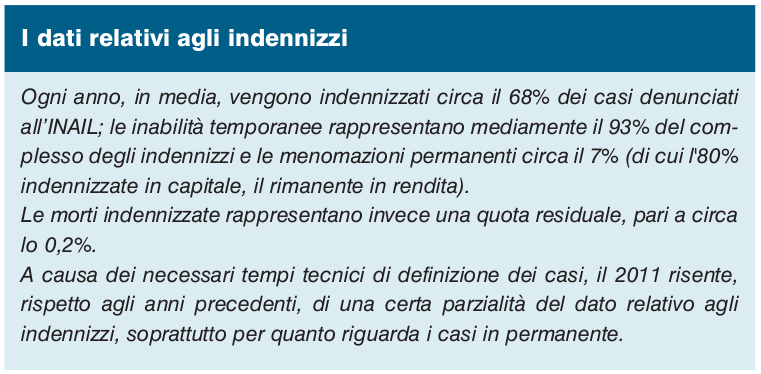
\includegraphics[scale=0.55]{images/analisiDiMercato/infortuniIndennizzi1}
\caption{Infortuni e indennizzi}
\end{figure}

\begin{figure}[H]
\centering
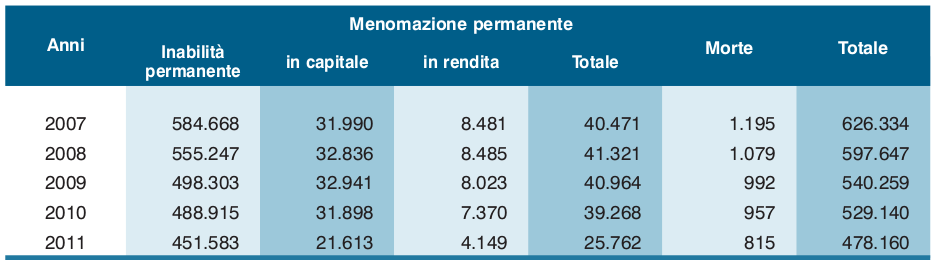
\includegraphics[scale=0.55]{images/analisiDiMercato/infortuniIndennizzi2}
\caption{Infortuni indennizzati nel quinquennio 2007-2011 per tutte le gestioni}
\end{figure}




\ \ \
\section{Osservazioni sui bilanci}
Dai bilanci Inail sugli infortuni sul lavoro riportati nelle sezioni precedenti, è possibile effettuare un'attenta lettura nel dettaglio, così da ricavare delle importanti osservazioni utili per capire come meglio sviluppare e incentrare il progetto Woty.\\
In primo luogo infatti è possibile comprendere quali siano i settori lavorativi più a rischio infortuni sul lavoro, nei quali il software Woty potrebbe avere una maggiore e più facile diffusione; e in secondo luogo è possibile comprendere quali siano le fasce di popolazione più a rischio infortuni, distinte per età, sesso e nazionalità.\\
E' molto importante infatti adempiere ad uno sviluppo \virgolette{mirato}, in particolar modo nella prima fase di sviluppo e di distribuzione del software, così da poter minimizarre i fattori di rischio iniziali.\\


\subsection{Woty: quali settori e attività lavorativi?}
Dai dati Inail relativi agli infortuni sul lavoro nell'ultimo decennio, si evince che la graduatoria dei settori lavorativi per il maggior numero di infortuni, vede al primo posto il settore dei \textbf{Servizi} che dal 2002 registra ogni anno più di 400.000 casi ( 450.000 casi nel 2002 - 416.000 casi nel 2011).\\
Al secondo posto troviamo il settore dell' \textbf{Industria} che registra una media di 350.000 casi nell'ultimo decennio. Gli infortuni in questo settore sono però in costante dimunizione e sono passati dai 460.000 casi nel 2002 ai 260.000 casi nel 2011.\\
Al terzo posto si classifica il settore dell' \textbf{Agricoltura} con una media di 50.000 casi all'anno. Anche in questo settore il numero è in lieve ma continua diminuzione registrando una variazione di circa 20.000 casi nell'ultimo decennio: 73.000 casi nel 2002 e 46.000 casi nel 2011.\\

Da ciò è possibile ricavare come i settori più indirizzati per lo sviluppo e diffusione di Woty sono i settori dei Servizi e dell'Industria, in quanto in questi due settori avviene il 90\% dei casi di infortuni.\\
Più nel dettaglio, osservando i dati Inail sugli infortuni per singola attività registrati nel 2011, nel settore dei servizi ad avere i valori più alti di infortuni sono le attività del \textbf{commercio} e dei \textbf{trasporti e comunicazioni}, mentre nel settore dell'industria le attività con i maggiori valori di infortuni sono quelle delle \textbf{costruzioni} e della \textbf{metallurgia}.\\
Ne consegue che saranno queste le attività lavorative verso le quali Woty dovrà indirizzarsi per poter avere una maggiore e più facile diffusione del software limitando i rischi di fallimento.\\


Tra le attività individuate come più adatte per l'utilizzo del software Woty, possiamo evidenziare come al loro interno siano presenti sia lavoratori con postazione fissa, sia lavoratori in mobilità; pertanto la piattaforma Woty potrà essere sfruttata nella sua interezza risultando così idonea agli ambiti di applicazione:\\
- per i lavoratori che dispongono di postazione fissa potrà essere utilizzato l'applicativo Woty desktop raggiungibile tramite dispositivi pc o notebook utilizzando un normale browser di navigazione internet\\
- per i lavoratori in mobilità presenti in ampia misura per esempio nei settori dei trasporti e del commercio, potrà essere utilizzato l'applicativo Woty mobile, che attraverso l'app permette l'utilizzo della piattaforma Woty direttamente da dispositivi mobili.



\subsection{Woty: quali età nei lavoratori?}
Osservando i dati relativi agli infortuni sul lavoro 2011, in relazione alle età dei lavoratori interessati, è possibile notare come ad essere più colpiti siano gli occupati con età comprese tra i 35 e 49 anni con ben 340.000 casi registrati nell'anno 2011.
Al secondo posto troviamo invece gli occupati con età inferionre ai 34 anni con ben 250.000 casi registrati nell'anno 2011.\\
Questi dati risultano essere favorevoli per la diffusione e un buon utilizzo del sistema Woty, in quanto essendo questa piattaforma molto innovativa e tecnologica, è più facilmente utilizzabile da parte di lavoratori appartenenti alla fascia d'età più giovane.\\
E' facilmente intuibile infatti che un occupato di età giovanile sia più indicato all'utilizzo delle tecnologie innovative, quali l'uso costante del pc oppure l'uso di cellulari smartphone con applicazioni innovative.



\subsection{Woty: lavoratori stranieri?}
Dai valori Inail sulla percentuale di lavoratori stranieri nel 2011, è emerso che ammontano a circa 3 milioni i lavoratori di nazionalità straniera presenti nel nostro, e sempre nel 2011 si sono registrati circa 115.000 casi di infortuni sul lavoro da parte di questi lavoratori, cioè il 15\% degli infortuni complessivi.\\
I valori risultano essere sufficientemente alti da far si che questa fascia di lavoratori debba essere presa in considerazione in ambito di sviluppo e diffusione della piattaforma Woty.\\
Deve essere presa in considerazione quindi l'utilizzo di Woty anche da parte di lavoratori stranieri e quindi il software dovrà supportare degli adeguati multilingua per permetterne un utilizzo più esteso, questo in previsione anche di una diffusione del software su scala internazionale.





\url{http://www.inail.it/Portale/appmanager/portale/desktop?_nfpb=true&_pageLabel=PAGE_SALASTAMPA&nextPage=Prodotti/Dossier_e_Speciali/SPECIALE_RAPPORTO_ANNUALE_2011/index.jsp}

















%--------------------------- CONCORRENZA

\newpage

\chapter{Concorrenza}

\section{Legislazione Vigente}

Con il decreto legislativo d.lgs. 626/94 si è andato ad approfondire quello che è l'ambito della sicurezza aziendale, introducendo tutta una nuova serie di obblighi per datori di lavoro e dipendenti. Tra questi obblighi possiamo trovare la necessità di formare tutti i collaboratori dell'azienda sui principali fattori di rischio, sulla prevenzione e sul primo soccorso, fino ad arrivare a nozioni più specialistiche riguardanti il tipo di azienda cui si appartiene e secondo la mansione che si ricopre.\\
Questa cosiddetta \virgolette{legge 626} è stata ora sostituita con il D.lgs. 81/2008 o \textit{Testo unico} sulla sicurezza sul lavoro ampliando notevolmente il carico di obblighi riguardanti l'informazione sulla sicurezza e la preparazione in suddetto ambito.\\
Per adeguare la propria azienda a questi standard ed essere in regola è necessario far seguire ai propri dipendenti dei corsi specifici. Questi corsi, se certificati, possono essere seguiti online, tenuti da terze parti o organizzati in azienda da personale addetto.\\
Woty intende quindi prendere parte all'ambito didattico per la sicurezza sostituendosi a uno di questi corsi.


\section{Concorrenza}

La formazione nel campo della sicurezza è trattata da una moltitudine di enti, associazioni, società private sia in ambito nazionale, sia in quello europeo. Certi di questi corsi sono gratuiti e questo può complicare la
commercializzazione del nostro prodotto.\\

Alcuni dei criteri presi in considerazione per valutare i corsi sono:

\begin{itemize}
	\item \textbf{Ambito} (nazionale, europeo)
	\item \textbf{Costo} (gratuito, a pagamento, prezzo per dipendente, etc.)
	\item \textbf{Locazione} (in sede, sede esterna, online, dispositivo mobile, etc.)
	\item \textbf{Localizzazione} (inglese, italiano, etc.)
	\item \textbf{Durata/Distribuzione oraria}
	\item \textbf{Utilizzo di Gamification} (peculiarità del nostro software)
\end{itemize}

Analizziamo quindi quali possono essere le principali minacce alla commercializzazione del nostro prodotto:


\begin{itemize}
	\item European Agency for Safety and Health at Work (EU-OSHA) (\url{http://osha.europa.eu})
		\begin{itemize}
			\item \url{http://www.healthy-workplaces.eu/it/hw2012}
			\item \url{http://www.healthy-workplaces.eu/it/media/ipad-app}
			\item \url{http://www.oiraproject.eu/}
		\end{itemize}
	\item INAIL (\url{http://www.ispesl.it/ew/ec2012/})
	\item PMI Servizi (\url{http://www.pmiservizi.it/corsi})
		\begin{itemize}
			\item Quotidiano Sicurezza (\url{http://itunes.apple.com/it/app/quotidiano-sicurezza/id419112770?mt=8})
		\end{itemize}
	\item ANFOS (Associazione Nazionale Formatori della Sicurezza sul Lavoro) (\url{http://www.anfos.it})
\end{itemize}

Vediamole ora nel dettaglio.

\section*{European Agency for Safety and Health at Work (EU-OSHA)}

L'agenzia europea per la salute e la sicurezza sul lavoro è la principale autorità in ambito europeo ed è una prolifica fonte di iniziative e progetti.\\
Gran parte delle risorse di quest'organizzazione è dedicata alla raccolta dati e alla pianificazione di convegni, attività che non minacciano la commercializzazione del nostro prodotto. Tuttavia l'organizzazione sfrutta una serie di partner localizzati nei principali paesi europei per l'organizzazione di corsi (fare riferimento a INAIL per l'analisi di questo punto) e inoltre sviluppa una serie di progetti, tra cui delle applicazioni online o per dispositivi mobile che potrebbero avere delle ripercussioni sul nostro prodotto. Analizziamole:

\begin{itemize}
	\item \textbf{Lavorare insieme per la prevenzione dei rischi} (\url{http://www.healthy-workplaces.eu/it/hw2012}) è una campagna che tratta nozioni di sicurezza e si presta anche come autovalutazione per aziende e dipendenti sulle sue principali tematiche. Questo sito online gratuito e localizzato in italiano non costituisce alcuna minaccia poiché fornisce solamente nozioni, ma non è regolamentato e non fornisce nessuna certificazione. Non può quindi sostituire un corso certificato.
	
	\item \textbf{Lavoriamo insieme – Campagna Ambienti di lavoro sani e sicuri} (\url{http://www.healthy-workplaces.eu/it/media/ipad-app}) è una delle pochissime applicazioni per dispositivi mobile che tratta l'argomento della sicurezza. Applicazione realizzata a seguito della campagna precedente. Non costituisce una minaccia poiché non permette la certificazione del dipendente.

	\item \textbf{Online Interactive Risk Assessment project} (\url{http://www.oiraproject.eu/}) web application in ambito della
sicurezza. Volge principalmente l'attenzione all'autovalutazione del proprio ambiente di lavoro e non offre certificazioni, quindi non rappresenta una minaccia.

\end{itemize}

\section*{INAIL}

Istituto Nazionale Assicurazione contro gli Infortuni sul Lavoro è il portavoce con sede nazionale delle principali iniziative organizzate dall'EU-OSHA. Oltre a campagne e seminari come \virgolette{Lavoriamo insieme per la prevenzione dei rischi}, che non intaccano il nostro mercato, l'INAIL organizza anche corsi e/o altre iniziative sulla sicurezza che portano a certificazione i partecipanti. Pur sembrando quindi una minaccia, classificheremo l'INAIL come opportunità poiché offre la possibilità di segnalare iniziative sulla sicurezza degne di nota di cui quest'ente si farà poi portavoce, fungendo da nostro partner/ente pubblicitario anziché competitor.

\section*{PMI Servizi}

Società di servizi per le piccole e medie imprese che si occupa di corsi di formazione per il personale aziendale.\\
Offre una varia gamma di corsi proprietari gratuiti online e offre la possibilità di ottenere un attestato a norma di legge il quale però è a pagamento. Essendo un servizio italiano online, il corso è in lingua italiana e frequentabile gratuitamente a qualsiasi orario da chiunque in possesso di un computer o di un dispositivo mobile.\\
Per gli esami il PMI Servizi è affiliato ad ANFOS e si rifà al suo listino prezzi.\\
Questa società offre inoltre \virgolette{Quotidiano Sicurezza} una notevole app per dispositivi mobile che offre nozioni, notizie, video guide, etc. sulla sicurezza nel lavoro. Nonostante non sia una minaccia per la nostra applicazione, quest'app deve essere monitorata. In caso gli sviluppatori aggiungano nuove funzionalità (ad esempio la possibilità di ottenere certificazioni a norma di legge tramite esami online) potrebbe divenire una potenziale minaccia.

\section*{Associazione Nazionale Formatori della Sicurezza sul Lavoro (ANFOS)}

Principale società italiana dedicata alla sicurezza sul lavoro. Offre una vasta gamma di servizi che spaziano dai corsi in aula a quelli online. Offre inoltre la possibilità di certificare i lavoratori a norma di legge.\\
Con questi servizi e oltre 560 sedi sul territorio l'ANFOS rappresenta il nostro maggior competitor.\\

Analizziamo ora le sue offerte per singolo individuo:

\begin{longtable}{ | l | r |}
\caption{Offerte ANFOS}\\
\hline
\endfirsthead
\multicolumn{2}{r}{\textit{(Continua alla pagina successiva)}}
\endfoot
\multicolumn{2}{l}{\textit{(Continua dalla pagina precedente)}}
\endhead
\hline
\endlastfoot
\textbf{Corso} \ & \textbf{Prezzo}\\
\hline
\rule[-2mm]{0mm}{0.7cm}
Corso formazione datore di lavoro quale R.S.P.P. modulo 1 e 2 & 80,00\EUR + Iva \\
\hline
\rule[-2mm]{0mm}{0.7cm}
Corso formazione Antincendio & 110,00\EUR + Iva \\
\hline
\rule[-2mm]{0mm}{0.7cm}
Corso per addetti al servizio aziendale di primo soccorso e gestione delle emergenze & 130,00\EUR + Iva \\
\hline
\rule[-2mm]{0mm}{0.7cm}
Corso aggiornamento addetto al servizio di primo soccorso & 70,00\EUR + Iva \\
\hline
\rule[-2mm]{0mm}{0.7cm}
Corso RLS & 200,00\EUR + Iva \\
\hline
\rule[-2mm]{0mm}{0.7cm}
Corso di formazione generale ed informazione lavoratore & 35,00\EUR + Iva \\
\hline
\rule[-2mm]{0mm}{0.7cm}
Corso formazione Carrellisti (Mulettisti) & 85,00\EUR + Iva \\
\hline
\rule[-2mm]{0mm}{0.7cm}
Corso di formazione per ricoprire il ruolo di Preposto & 110,00\EUR + Iva \\
\hline
\rule[-2mm]{0mm}{0.7cm}
Corso primo ingresso in cantiere per i lavoratori edili & 140,00\EUR + Iva \\
\hline
\rule[-2mm]{0mm}{0.7cm}
Corso Aggiornamento RLS & 100,00\EUR + Iva \\
\hline
\rule[-2mm]{0mm}{0.7cm}
Corso di Aggiornamento R.S.P.P. & 9,00\EUR + Iva \\
\hline
\rule[-2mm]{0mm}{0.7cm}
Corso rischio stress lavoro correlato per lavoratori R.S.P.P. & 35,00\EUR + Iva \\
\hline
\rule[-2mm]{0mm}{0.7cm}
Corso rischio stress lavoro correlato per professionisti & 120,00\EUR + Iva \\
\hline
\rule[-2mm]{0mm}{0.7cm}
Corso di aggiornamento Addetto Antincendio (rischio basso) & 70,00\EUR + Iva \\
\hline
\rule[-2mm]{0mm}{0.7cm}
Corso di formazione per i responsabili dell'industria alimentare & 35,00\EUR + Iva \\
\hline
\rule[-2mm]{0mm}{0.7cm}
Corso formazione personale qualificato (che manipola alimenti e bevande) & 35,00\EUR + Iva \\
\hline
\rule[-2mm]{0mm}{0.7cm}
Corso formazione addetti industria alimentare (che non manipolano alimenti e bevande) & 35,00\EUR + Iva \\
\hline
\rule[-2mm]{0mm}{0.7cm}
Corso per Formatori & 200,00\EUR + Iva \\
\hline
\end{longtable}

I corsi sono compresi di esame/certificazione.\\

Pur tuttavia rappresentando il nostro maggior competitor, quest'organizzazione non dispone di un'applicazione mobile che intacchi il nostro mercato dei lavoratori in mobilità e richiede specificatamente il possesso di un computer, oppure la presenza in aula(durata del corso e distribuzione oraria variano da regione a regione e da ditta a ditta).

\section{Panoramica dei dati sui competitors}

Analizziamo ora i dati raccolti sui quattro possibili concorrenti:\\

L'offerta del proprio corso in italiano è un forte fattore discriminante per la scelta di un corso poiché quasi il 40\% dei lavoratori italiani non conosce la lingua inglese e solo il 10\% la conosce a sufficienza.

% inserire una figura
\begin{figure}[H]
\centering
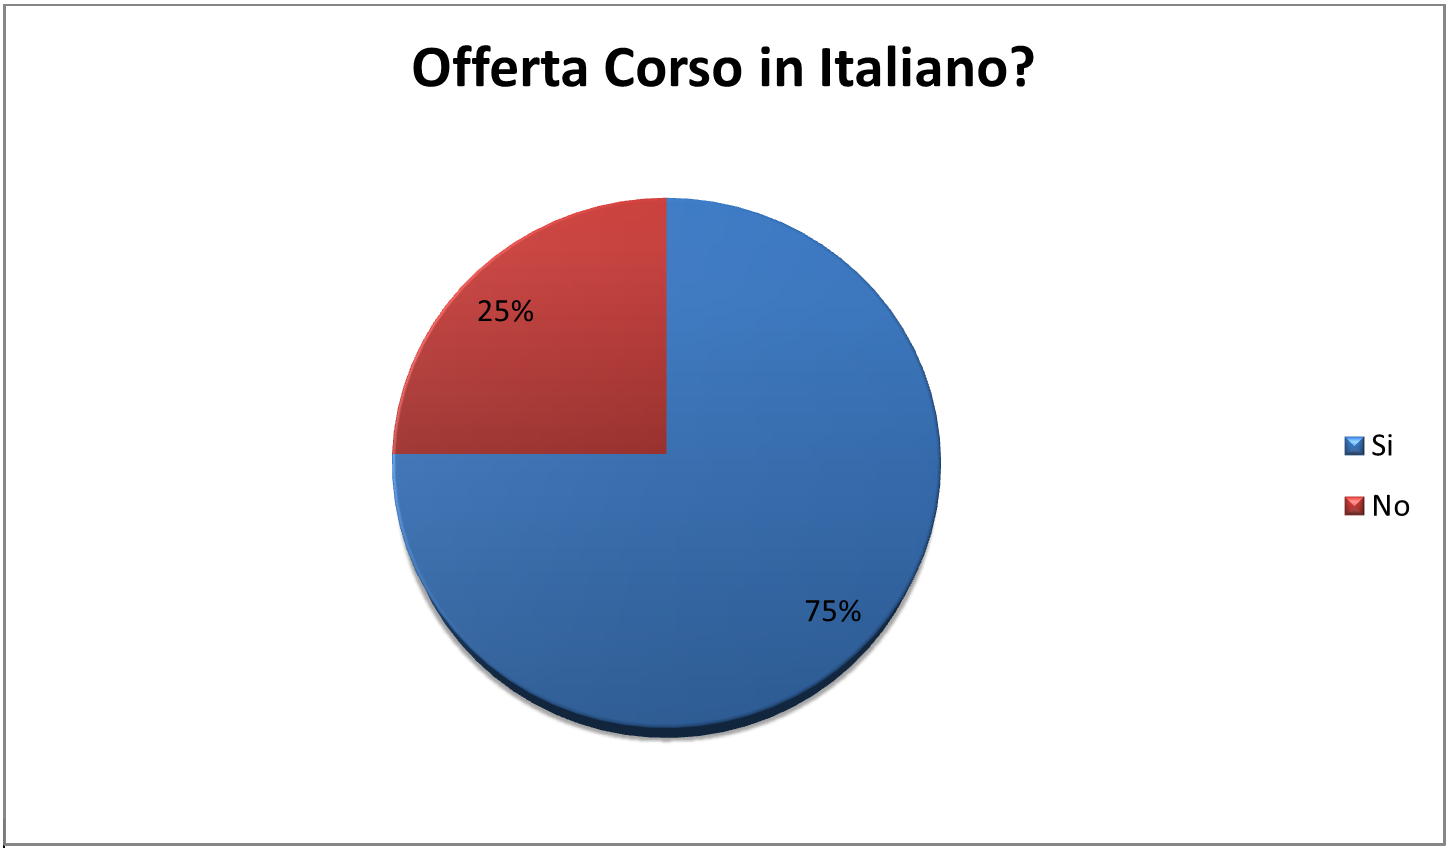
\includegraphics[scale=0.20]{images/graficiConcorrenza/corsoItaliano.png}
\caption{Offerta corso in italiano}
\end{figure}

Un altro importante fattore discriminante è il costo dei corsi.

% inserire una figura
\begin{figure}[H]
\centering
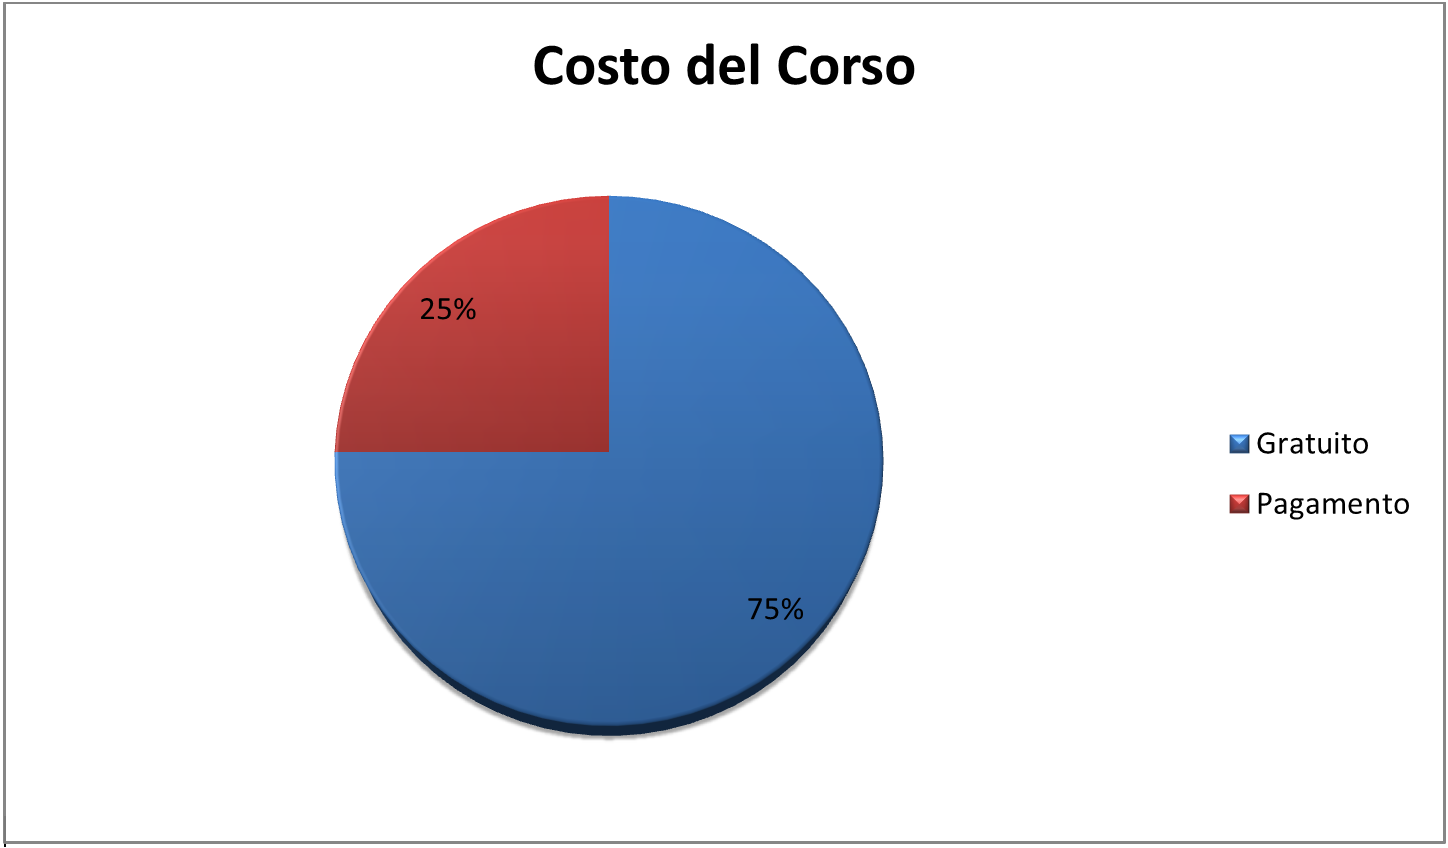
\includegraphics[scale=0.20]{images/graficiConcorrenza/costoCorso.png}
\caption{Costo del corso}
\end{figure}

Passiamo ora ad analizzare quanti offrono una certificazione riconosciuta.

% inserire una figura
\begin{figure}[H]
\centering
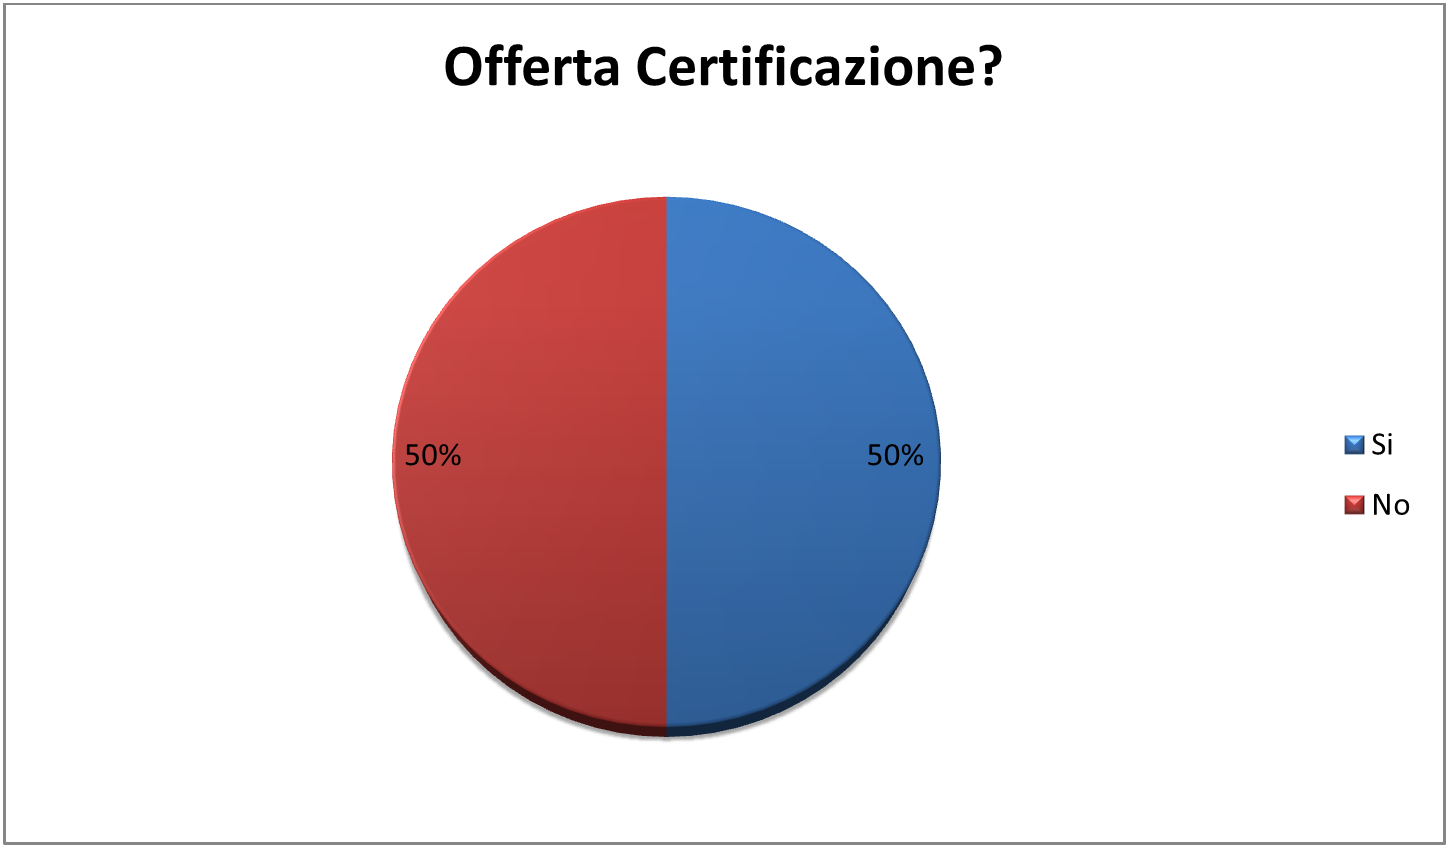
\includegraphics[scale=0.20]{images/graficiConcorrenza/offertaCertificazione.png}
\caption{Offerta certificazione}
\end{figure}

E infine analizziamo quanti di questi utilizzano principi di gamification nei propri corsi.

% inserire una figura
\begin{figure}[H]
\centering
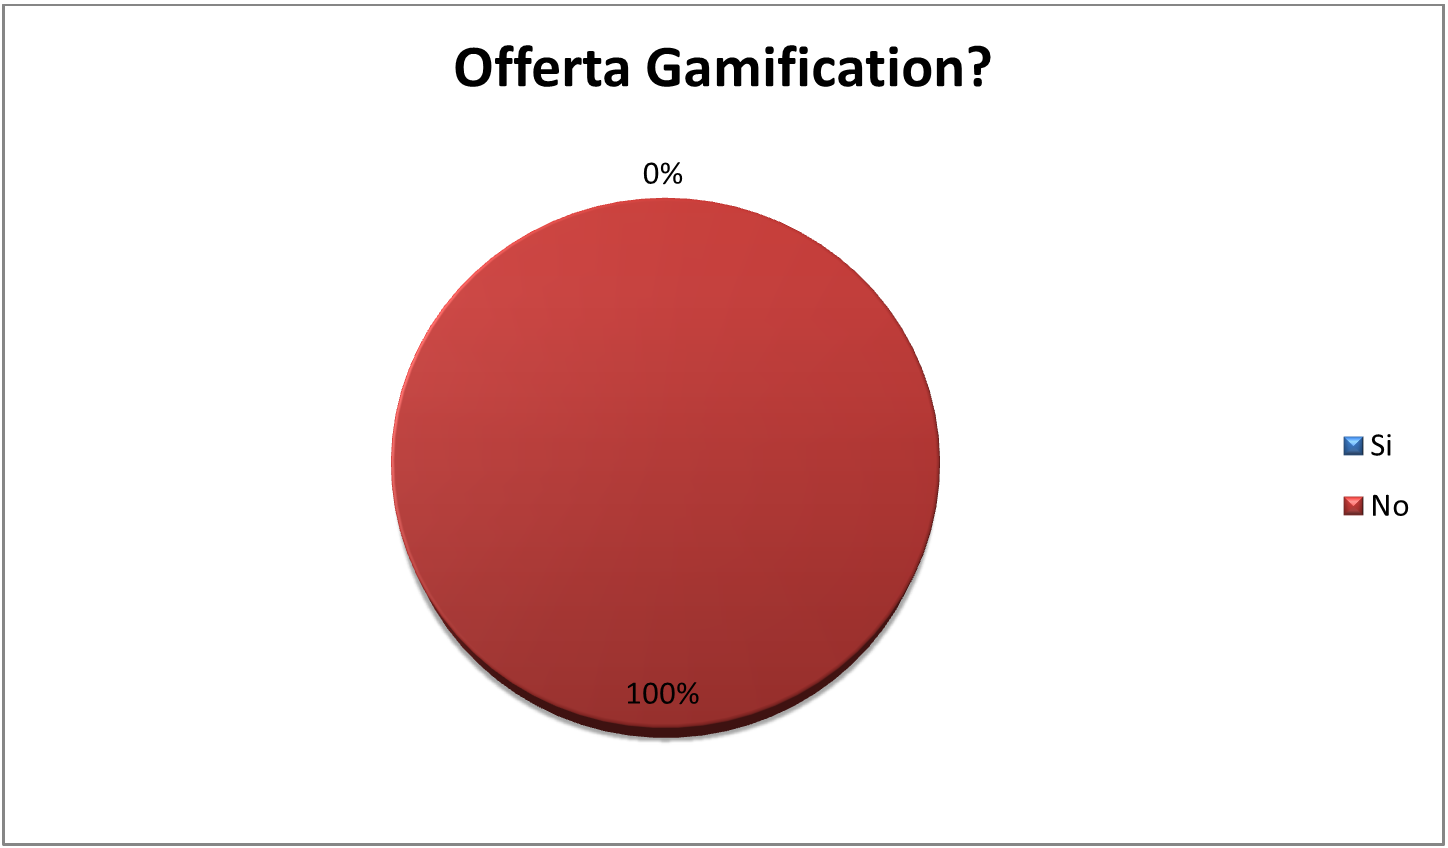
\includegraphics[scale=0.20]{images/graficiConcorrenza/principiGamification.png}
\caption{Uso di principi di Gamification}
\end{figure}

\section{Conclusioni}

Dai dati raccolti in precedenza, possiamo evincere le seguenti conclusioni:

\begin{enumerate}
	\item Nel mercato dei lavoratori in \textbf{mobilità} attualmente non abbiamo rivali. Woty permettere di coprire questa nicchia in maniera esclusiva. È tuttavia consigliato il monitoraggio delle due applicazioni \textbf{mobile} rilevate o lo sviluppo di nuove app per impedire di perdere questa egemonia.
	
	\item In ambito desktop o in quello dei corsi frontali il nostro unico competitor è \textbf{ANFOS} (poiché l'altro possibile concorrente si rifà a quest'ultimo per i test e il listino prezzi). Finché la nostra offerta sarà superiore in convenienza rispetto all'offerta di ANFOS risulterà unica poiché offre elementi di gamification, permette l'accesso al servizio anche ai lavoratori in mobilità e permette di evitare la perdita di giorni lavorativi per frequentare le lezioni frontali.
	
	\item Vista la grande diffusione di corsi gratuiti sulla sicurezza sul lavoro, è necessario che il nostro software rilasci attestati validi \textbf{certificati} a norma di decreto legislativo 81/2008 per essere commercializzato.
Ci si è dovuti quindi rivolgere al Ministero del Lavoro e delle Politiche Sociali per essere sottoposti a un  processo di certificazione. Una volta superato tuttavia è necessario pagare una tassa d'iscrizione annua pari 
a 1970\EUR + Iva.
Per ammortizzare questi o successivi costi richiesti in futuro, ci si affida alla possibilità di sfruttare fondi europei destinati a iniziative sulla sicurezza sul lavoro.
\\
\\
\red{umba prendi qualche spunto da questo pezzetto k avevo scritto io}\\
Vista la larga scala di indennizzi rilasciati dall'Inail sugli infortini sul lavoro, questo potrebbe essere motivante per poter prevedere anche una certificazione del software al ministero del lavoro a livello nazionale statale, venendo quindi riconosciuto come software certificato.\\
Tutto questo deve essere comunque collegato ad una buona diffusione iniziale del software così da permettere e garantire che il software abbia raggiunto un buon grado di maturità e sviluppo.\\
In seguito a questo potrebbe essere valutata la richiesta di eventuali incentivi statali per il mantenimento e supporto tecnico del software.


\end{enumerate}

\end{document}
